\documentclass{article}

% Language setting
% Replace `english' with e.g. `spanish' to change the document language
\usepackage[english]{babel}

% Set page size and margins
% Replace `letterpaper' with`a4paper' for UK/EU standard size
\usepackage[letterpaper,top=2cm,bottom=2cm,left=3cm,right=3cm,marginparwidth=1.75cm]{geometry}

% Useful packages
\usepackage{amsmath}
\usepackage{amssymb}
\usepackage{bbm}
\usepackage{graphicx}
\usepackage{enumitem}
\usepackage{cancel}
\usepackage[colorlinks=true, allcolors=blue]{hyperref}

\usepackage{hyperref}
\hypersetup{
    colorlinks=true,
    linkcolor=blue,
    filecolor=magenta,      
    urlcolor=cyan,
    pdftitle={137B HW 1 - KDEOSKAR},
    pdfpagemode=FullScreen,
    }

\urlstyle{same}

\usepackage{tikz-cd}

%%%%%%%%%%% Box pacakges and definitions %%%%%%%%%%%%%%
\usepackage[most]{tcolorbox}
\usepackage{xcolor}

% Define the colors
\definecolor{boxheader}{RGB}{0, 51, 102}  % Dark blue
\definecolor{boxfill}{RGB}{173, 216, 230}  % Light blue

% Define the tcolorbox environment
\newtcolorbox{mathdefinitionbox}[2][]{%
    colback=boxfill,   % Background color
    colframe=boxheader, % Border color
    fonttitle=\bfseries, % Bold title
    coltitle=white,     % Title text color
    title={#2},         % Title text
    enhanced,           % Enable advanced features
    attach boxed title to top left={yshift=-\tcboxedtitleheight/2}, % Center title
    boxrule=0.5mm,      % Border width
    sharp corners,      % Sharp corners for the box
    #1                  % Additional options
}
%%%%%%%%%%%%%%%%%%%%%%%%%

\newtcolorbox{dottedbox}[1][]{%
    colback=white,    % Background color
    colframe=white,    % Border color (to be overridden by dashrule)
    sharp corners,     % Sharp corners for the box
    boxrule=0pt,       % No actual border, as it will be drawn with dashrule
    boxsep=5pt,        % Padding inside the box
    enhanced,          % Enable advanced features
    overlay={\draw[dashed, thin, black, dash pattern=on \pgflinewidth off \pgflinewidth, line cap=rect] (frame.south west) rectangle (frame.north east);}, % Dotted line
    #1                 % Additional options
}

\usepackage{biblatex}
\addbibresource{sample.bib}


%%%%%%%%%%% New Commands %%%%%%%%%%%%%%
\newcommand*{\T}{\mathcal T}
\newcommand*{\cl}{\text cl}


\newcommand{\ket}[1]{|#1 \rangle}
\newcommand{\bra}[1]{\langle #1|}
\newcommand{\inner}[2]{\langle #1 | #2 \rangle}
\newcommand{\mean}[1]{\langle #1 \rangle}
\newcommand{\R}{\mathbb{R}}
\newcommand{\C}{\mathbb{C}}
\newcommand{\V}{\mathbb{V}}
\newcommand{\Hilbert}{\mathcal{H}}
\newcommand{\oper}{\hat{\Omega}}
\newcommand{\lam}{\hat{\Lambda}}

\newcommand{\bigslant}[2]{{\raisebox{.2em}{$#1$}\left/\raisebox{-.2em}{$#2$}\right.}}
\newcommand{\restr}[2]{{% we make the whole thing an ordinary symbol
  \left.\kern-\nulldelimiterspace % automatically resize the bar with \right
  #1 % the function
  \vphantom{\big|} % pretend it's a little taller at normal size
  \right|_{#2} % this is the delimiter
  }}
%%%%%%%%%%%%%%%%%%%%%%%%%%%%%%%%%%%%%%%


\tcbset{theostyle/.style={
    enhanced,
    sharp corners,
    attach boxed title to top left={
      xshift=-1mm,
      yshift=-4mm,
      yshifttext=-1mm
    },
    top=1.5ex,
    colback=white,
    colframe=blue!75!black,
    fonttitle=\bfseries,
    boxed title style={
      sharp corners,
    size=small,
    colback=blue!75!black,
    colframe=blue!75!black,
  } 
}}

\newtcbtheorem[number within=section]{Theorem}{Theorem}{%
  theostyle
}{thm}

\newtcbtheorem[number within=section]{Definition}{Definition}{%
  theostyle
}{def}



\title{Physics 137B Homework 1}
\author{Keshav Balwant Deoskar}

\begin{document}
\maketitle

% \vskip 0.5cm
% \pagebreak 

%%%%%%%%%%%%%%%%%%%%%%%%%%%%%%%%%%%%%%%%%%%%%%%%%%%%%%%%%%%%%%%%%
\begin{dottedbox}
\textbf{Q1. Rotations about the z-axis:} 
\begin{enumerate}[label=(\alph*)]
  \item Let $\hat{R}_{z}(\delta)$ be the operator that rotates a function about the $z-$axis by an angle $\delta$. It is defined by 
  \[ \hat{R}_z (\delta) \psi(r, \theta, \phi) = \psi'(r, \theta, \phi) = \psi(r, \theta, \phi - \delta) \;\;\;(1) \]

  For an infinitessimal value of $\delta$, show that 
  \[ \hat{R}_z(\delta) \approx 1 - \frac{i\delta}{\hbar}\hat{L}_z \]\
  where $\hat{L}_z$ is the angular momentum operator about the z-axis.

  \vskip 0.5cm
  \item Using the taylor expansion for the right hand side of Equation (1), show that in general the operator $\hat{R}_{z}(\delta)$ is given by 
  \[ \hat{R}_{z}(\delta) = \exp\left[ -\frac{i\delta}{\hbar} \hat{L}_z \right] \]

  \vskip 0.5cm
  \item Consider a small value of $\delta$, and evaluate the action of $\hat{R}_z(\delta)$ on the position 3D vector 
  \[ \vec{r} = \begin{pmatrix}
    x \\
    y \\
    z
  \end{pmatrix} \]

  Draw a picture depicting this transformation and reconcile it with your result for $\hat{R}_z(\delta) \vec{r}$.

  \vskip 0.5cm
  \item We can readily write down the rotation operator for spin$-1/2$ particles, by replacing $\hat{L}_z$ with $\hat{S}_z = \frac{\hbar}{2} \sigma_z$
  where 
  \[ \sigma_z = \begin{pmatrix}
    1 & 0 \\
    0 & -1
  \end{pmatrix} \]
  is the Pauli matrix. With this, we find the rotation operator for a spin$-1/2$ particle to be 
  \[ \hat{R}_{z, 1/2}(\delta) = \exp\left[ -\frac{i \delta}{2} \sigma_z \right] \]
  Using the Taylor series of this operator and the fact $\sigma_z^2 = 1$, write $\hat{R}_{z, 1/2}(\delta) $ explicitly as a two by two matrix. [Note:
  although you are using the Taylor series to arrive at your final expression, the final result should hold for any real value of $\delta$]

  \item Let $\chi_+^(z)$ be an eigenvector of $\sigma_z$ with eigenvalue $+1$. That is, $\sigma_z \chi_+^{(z)} = \chi_+^{(z)}$. Evaluate $\hat{R}_z(\delta) \chi_+^{(z)}$. Explain your result.
  
  \item Find the normalized eigenvectors $(\chi_{\pm}^{(z)})$ with eigenvalues $\pm$ of the $\sigma_y$ Pauli matrix
  \[ \sigma_y = \begin{pmatrix}
    0 & -i \\
    i & 0 
  \end{pmatrix} \]

  \item Evaluate the action of the matrix you got above on the $\chi_+^{(y)}$, i.e. $\hat{R}_z(\delta)(\chi_+^{(y)})$. Explain your result.
\end{enumerate}
\end{dottedbox}
%%%%%%%%%%%%%%%%%%%%%%%%%%%%%%%%%%%%%%%%%%%%%%%%%%%%%%%%%%%%%%%%%

\vskip 0.5cm
\underline{\textbf{Solutions:}} 

\begin{enumerate}[label=(\alph*)]
  \item We define $\hat{R}_z(\delta)$ as 
  \[ \hat{R}_z (\delta) \psi(r, \theta, \phi) = \psi(r, \theta, \phi - \delta) \]
  
  Taylor expanding in terms of $\phi$, we have 
  \begin{align*}
    \psi(r, \theta, \phi - \delta) &= \psi(r, \theta, \phi) - \delta \frac{\partial \psi}{\partial \phi} + \cdots
  \end{align*}
  and the Angular Momentum operator about the $z-$axis can be expressed as 
  \begin{align*}
    \hat{L}_z &= -i\hbar \frac{\partial}{\partial \phi} \\
    \implies \frac{\partial}{\partial \phi} &= \frac{i\hat{L}_z}{\hbar}
  \end{align*}
  
  Thus, 
  \begin{align*}
    \psi(r, \theta, \phi - \delta) = \psi(r, \theta, \phi) - \frac{i\delta \hat{L}_z}{\hbar}\psi(r, \theta, \phi) + \cdots
  \end{align*}
  That is, to first order approximation, we have 
  \[ \boxed{\hat{R}_z(\theta) \psi(r, \theta, \phi) = 1 - \frac{i \delta \hat{L}_z}{\hbar} \psi(r, \theta, \phi)} \]

  \vskip 1cm
  \item Using the Taylor expansion
  \begin{align*}
    \psi(r, \theta, \phi - \delta) &= \psi - \delta \frac{\partial \psi}{\partial \phi} + \frac{1}{2!} \frac{\partial^2 \psi}{\partial \phi^2} \delta^2 + \cdots \\
    \implies \hat{R}_z(\delta) \psi(r, \theta, \phi) &= \left(\mathbf{1} - \delta \frac{\partial}{\partial \phi} + \frac{1}{2!} \frac{\partial^2}{\partial \phi^2} \delta^2 + \cdots  \right) \psi(r, \theta, \phi) \\
    \implies \hat{R}_z(\delta)\psi(r, \theta, \phi) &= \left( \mathbf{1} - \frac{i \delta}{\hbar}\hat{L}_z + \cdots \right) \psi(r, \theta, \phi) \\
    \implies \hat{R}_z(\delta) &=  \sum_{n = 0} \frac{1}{n!} \left(-\frac{i \delta}{\hbar} \hat{L}_z \right)^n 
  \end{align*}
  Therefore, 
  \[ \boxed{ \hat{R}_z(\delta) = \exp\left[ -\frac{i \delta}{\hbar} \hat{L}_z \right] } \]


  \vskip 1cm
  \item We consider an arbitrary 3D position vector 
  \begin{equation*}
    \vec{r} = 
  \begin{pmatrix}
    x \\
    y \\
    z
  \end{pmatrix} 
  = 
  \begin{pmatrix}
    r \sin(\theta) \cos(\phi) \\
    r \sin(\theta) \sin(\phi) \\
    r \cos(\theta) 
  \end{pmatrix} 
  \end{equation*}

  Now, acting on this vector with $\hat{R}_z(\delta)$ has the effect of carrying out the transformation $\phi \rightarrow \phi - \delta$, so  

  \begin{align*}
    \vec{r}' &= 
    \begin{pmatrix}
      r \sin(\theta) \cos(\phi - \delta) \\
      r \sin(\theta) \sin(\phi - \delta) \\
      r \cos(\theta) 
    \end{pmatrix} \\
    &= \begin{pmatrix}
      r \sin(\theta) \left[ \cos(\phi)\cos(\delta) + \sin(\phi)\sin(\delta)  \right]\\
      r \sin(\theta) \left[\sin(\phi)\cos(\delta) - \cos(\phi)\sin(\delta) \right] \\
      r \cos(\theta) 
    \end{pmatrix}
  \end{align*}
  Since $\delta$ is small, $\cos(\delta) \approx 1$ and $\sin(\delta) \approx \delta$. So, 

  \begin{align*}
    \vec{r}' &= \begin{pmatrix}
      r \sin(\theta) [\cos(\phi) \cdot 1 + \sin(\phi) \cdot \delta] \\
      r \sin(\theta) \left[ \sin(\phi) \cdot 1 - \cos(\phi)\cdot \delta \right] \\
      r \cos(\theta) 
    \end{pmatrix} \\
    &= \begin{pmatrix}
      r\sin(\theta)\cos(\phi) + \delta \cdot r\sin(\theta)\cos(\phi) \\
      r\sin(\theta)\sin(\phi) - \delta \cdot r\sin(\theta)\cos(\phi) \\
      r\cos(\theta)
    \end{pmatrix} \\
    &= \begin{pmatrix}
      x + \delta y \\
      y - \delta x \\
      z
    \end{pmatrix}
  \end{align*} 
  Thus, applying the $\hat{R}_z(\delta)$ operator with a small value of $\delta$ has the effect of the transformation:
  \begin{align*}
    \begin{array}{cc}
      x \\ y \\ z
    \end{array} \rightarrow \begin{array}{cc}
      x + \delta y \\ y - \delta x \\ z
    \end{array}
  \end{align*}
  
  \vskip 0.5cm
  \begin{center}
    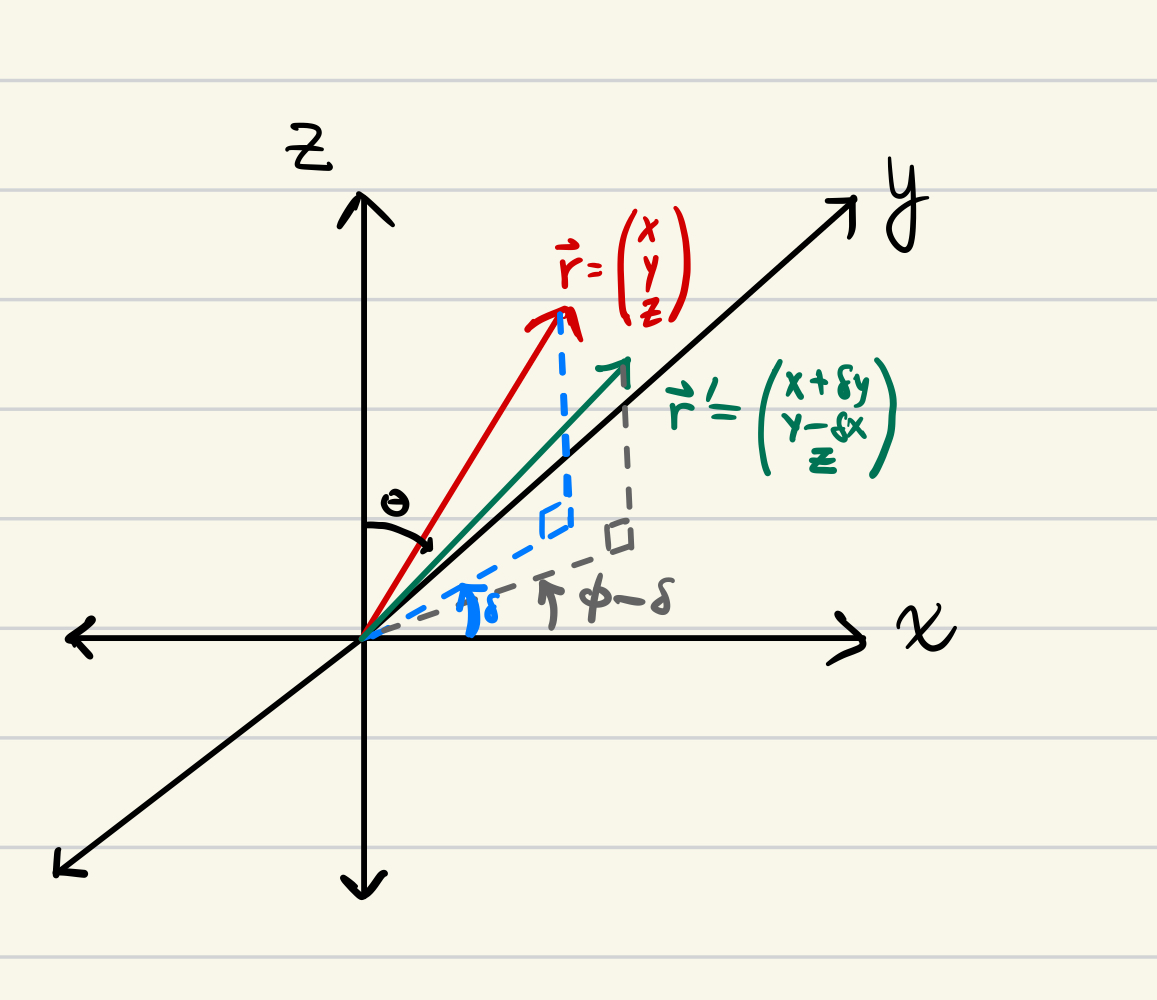
\includegraphics[scale=0.20]{Q1.jpg}
  \end{center}

  \vskip 1cm
  \item For a spin-1/2 particle, we have 
  \[ \hat{R}_{z, 1/2} (\delta) = \exp \left[ -\frac{i \delta}{2} \sigma_z \right] \]

  We now want to explicitly find the matrix representation of this operator, using the taylor series and the fact that $\sigma_z^2 = \mathbbm{1}$.

  Now,
  \begin{align*}
    \hat{R}_{z, 1/2} (\delta) &= \exp \left[ -\frac{i \delta}{2} \sigma_z \right] \\
    &= \sum_{n = 0}^{\infty} \frac{1}{n!} \cdot \left( -\frac{i \delta}{2} \sigma_z  \right)^n
  \end{align*}
  and 
  \begin{align*}
    &\sigma_z^2 = \mathbbm{1} \implies \sigma_z^{2k} = \mathbbm{1} \\
    &\sigma_z^2 = \mathbbm{1} \implies \sigma_z^{2k+1} = \sigma_z \\
  \end{align*}

  So, 
  \begin{align*}
    \hat{R}_{z, 1/2} (\delta) &= \sum_{k \in \mathbb{N}} \left[\frac{1}{(2k)!} \left(-\frac{i\delta}{2}\right)^{2k} \mathbbm{1}\right] + \sum_{k \in \mathbb{N}} \left[\frac{1}{(2k+1)!} \left(-\frac{i\delta}{2}\right)^{2k+1} \sigma_z\right] \\
    &= \left[ \sum_{k \in \mathbb{N}} \frac{1}{(2k)!} \left(-\frac{i\delta}{2}\right)^{2k}  \right] \mathbbm{1} + \left[ \sum_{k \in \mathbb{N}} \frac{1}{(2k+1)!} \left(-\frac{i\delta}{2}\right)^{2k+1} \right] \sigma_z 
  \end{align*}

  For the sake of convenience, let's denote the two sums as 
  \begin{align*}
    A &\equiv \sum_{k \in \mathbb{N}} \frac{1}{(2k)!} \left(-\frac{i\delta}{2}\right)^{2k}  \\
    B &\equiv  \sum_{k \in \mathbb{N}} \frac{1}{(2k+1)!} \left(-\frac{i\delta}{2}\right)^{2k+1}
  \end{align*}

  Recall that the matrix representations of $\mathbbm{1}$ and $\sigma_z$ are 

  \begin{align*}
    \mathbbm{1} &= \begin{pmatrix}
      1 & 0 \\
      0 & 1
    \end{pmatrix} \\
    \sigma_z &= \begin{pmatrix}
      1 & 0 \\
      0 & -1 
    \end{pmatrix}
  \end{align*}

  Then,
  \begin{align*}
    \hat{R}_{z, 1/2} (\delta) &= A \mathbbm{1} + B \sigma_z \\
    &= \begin{pmatrix}
      A & 0 \\
      0 & A
    \end{pmatrix} + 
    \begin{pmatrix}
      B & 0 \\
      0 & -B
    \end{pmatrix} \\
    &= \begin{pmatrix}
      A + B & 0 \\
      0 & A - B
    \end{pmatrix}
  \end{align*}

  But notice that 
  \begin{align*}
    A + B &= \sum_{k \in \mathbb{N}}^{\infty} \frac{1}{k!} \left( -\frac{i \delta}{2} \right)^k \\
    &= e^{-\frac{i \delta}{2}}
  \end{align*}
  and 
  \begin{align*}
    A - B &= \sum_{k \in \mathbb{N}}^{\infty} \frac{1}{k!} \cdot (-1)^{k} \left( -\frac{i \delta}{2} \right)^k \\
    &= \sum_{k \in \mathbb{N}}^{\infty} \frac{1}{k!} \cdot \left( -1 \times -\frac{i \delta}{2} \right)^k \\
    &= \sum_{k \in \mathbb{N}}^{\infty} \frac{1}{k!} \left( \frac{i \delta}{2} \right)^k \\
    &= e^{+\frac{i \delta}{2}}
  \end{align*}

  Therefore, the final expression we get for the rotation operator is

  \[ \boxed{\hat{R}_z(\delta) = \begin{pmatrix}
    e^{-\frac{i \delta}{2}} & 0 \\
    0 &  e^{+\frac{i \delta}{2}}
  \end{pmatrix}} \]

  \vskip 0.5cm
  \item We let $\chi_+^{(z)}$ be the eigenvector of $\sigma_z$ having eigenvalue $+1$ i.e. $\sigma_z \chi_+^{(z)} = \chi_+^{(z)}$.
  
  \begin{align*}
    &\sigma_z \chi_+^{(z)} = \chi_+^{(z)} \\
    \implies &\begin{pmatrix}
      1 & 0 \\
      0 & -1
    \end{pmatrix} \begin{pmatrix}
      a \\
      b
    \end{pmatrix} = \begin{pmatrix}
      a \\
      b
    \end{pmatrix} \\
    \implies &\begin{cases}
      a = a \\
      b = -b
    \end{cases}
  \end{align*}
  So, $b = 0$ and $a$ can be any real number (before normalization), but as per convention let's choose $a = 1$. So,
  \[ \boxed{ \chi_+^{(z)} = \begin{pmatrix} 1 \\ 0 \end{pmatrix} } \]

  Applying the rotation operator then gives us 
  \begin{align*}
    \hat{R}_z(\delta) \chi_+^{(z)} &= \begin{pmatrix}
      e^{-i \delta / 2} & 0 \\
      0 & e^{+i \delta / 2}  
    \end{pmatrix} \begin{pmatrix}
      1 \\ 0
    \end{pmatrix} \\
    &= \begin{pmatrix}
      e^{-i \delta / 2} \\ 0
    \end{pmatrix} \\
    &= e^{- i \delta /2 } \begin{pmatrix}
      1 \\ 0
    \end{pmatrix}
  \end{align*}

  Thus, 
  \[ \boxed{\hat{R}_{z, 1/2}(\delta) \chi_+^{(z)} = e^{- i\delta /2} \chi_+^{(z)} }  \]

  So, applying the rotation matrix does not change the physical system, which makes sense. 

  \begin{align*}
    \sigma_z \left( \hat{R}_{z, 1/2}(\delta) \chi_+^{(z)} \right) &= \sigma_z \left( e^{- i\delta /2} \chi_+^{(z)} \right) \\
    &= e^{-i\delta /2} \left( \sigma_z \chi_+^{(z)} \right) \\
    &= e^{- i\delta /2} \chi_+^{(z)} \\
    &= \hat{R}_{z, 1/2}(\delta) \chi_+^{(z)}
  \end{align*}

  So, the rotated spinor is \emph{also} an eigenspinor of $\sigma_z$ with eigenvalue $+1$. Intuitively this makes sense, because $\chi_+^{(z)}$ was already completely "aligned" with the $z-$axis, so rotation about the $z-$axis should make no observable difference.

  \vskip 0.5cm
  \item We want to find the normalized eigenvectors $(\chi_{\pm}^{(y)})$ with eigenvalue $\pm 1$ of the $\sigma_y$ Pauli Matrix,
  \[ \sigma_y = \begin{pmatrix}
    0 & -i \\
    i & 0
  \end{pmatrix} \]

  Let $\chi = \begin{pmatrix}
    a \\ b
  \end{pmatrix}$ be an eigenvector of $\sigma_y$ with eigenvalue $\pm 1$. Then,

  \begin{align*}
    &\begin{pmatrix}
      0 & -i \\
      i & 0
    \end{pmatrix} \begin{pmatrix}
      a \\ b
    \end{pmatrix} = \pm \begin{pmatrix}
      a \\ b
    \end{pmatrix} \\
    \implies &\begin{pmatrix}
      -ib \\
      ia 
    \end{pmatrix} = \pm \begin{pmatrix}
      a \\ b
    \end{pmatrix}
  \end{align*}

  \underline{For the $+1$ case:}
  \begin{align*}
    -ib &= a \\
    ia &= b
  \end{align*}

  \begin{align*}
    \implies & -i(ia) = a \\
    \implies & \boxed{a = a}
  \end{align*}
  and 
  \begin{align*}
    b &= -\frac{1}{i}a \\
    \implies &\boxed{b = i a}
  \end{align*}
  i.e we can arbitrarily choose $a$, get $b$ from $b = ia$, and then normalize the spinor as $\chi^{\dagger} \chi = 1$. 
  
  We found that the $(+1)$-eigenspinor has the form $\chi_+^{(y)} = \begin{pmatrix}
    a \\
    ia 
  \end{pmatrix}$.

  \begin{align*}
    &(\chi_+^{(y)})^{\dagger} \chi_+^{(y)} = 1 \\
    \implies &\begin{pmatrix}
      a & -ia
    \end{pmatrix} \begin{pmatrix}
      a \\
      ia
    \end{pmatrix} = 1 \\
    \implies &a^2 + a^2 = 1 \\
    \implies &a^2 = \frac{1}{2} \\
    \implies &\boxed{a = \frac{1}{\sqrt{2}}}
  \end{align*}

  So, the $+1$ eigenspinor is 
  \[ \boxed{ \chi_+^{(y)} = \frac{1}{\sqrt{2}} \begin{pmatrix} 1 \\ i \end{pmatrix} } \]

  \underline{For the $-1$ case:}
  \begin{align*}
    -ib &= -a \\
    ia &= -b
  \end{align*}

  \begin{align*}
    \implies & i(-ia) = a \\
    \implies & \boxed{a = a}
  \end{align*}
  and 
  \begin{align*}
    \boxed{b = -ia}
  \end{align*}
  So, following the same argument as before, $(\chi_{-}^{(y)})^{\dagger} \chi_-^{(y)} = 1$ gives
  \begin{align*}
    &\begin{pmatrix}
      a & ia
    \end{pmatrix} \begin{pmatrix}
      a \\
      -ia
    \end{pmatrix} = 1 \\
    \implies &a^2 + a^2 = 1 \\
    \implies & \boxed{a = \frac{1}{\sqrt{2}}}
  \end{align*}

  So, the $(-1)$-eigenspinor is 
  \[ \boxed{ \chi_-^{(y)} = \frac{1}{\sqrt{2}} \begin{pmatrix} 1 \\ -i \end{pmatrix}  } \]

  \vskip 1cm
  \begin{dottedbox}
    To summarise, the normalized eigenspinors of the $\sigma_z$ Pauli matrix are $\chi_+^{(y)}$ and $\chi_-^{(y)}$ given by 
    \begin{align*}
      \chi_+^{(y)} &= \frac{1}{\sqrt{2}} \begin{pmatrix} 1 \\ i \end{pmatrix} \\
      \chi_+^{(y)} &= \frac{1}{\sqrt{2}} \begin{pmatrix} 1 \\ -i \end{pmatrix} 
    \end{align*}
  \end{dottedbox}
  
  \vskip 0.5cm 
  \item Now, let's evaluate the rotation matrix on $\chi_+^{(y)}$.
  
  \begin{align*}
    \hat{R}_z(\delta)\chi_+^{(y)} &= \begin{pmatrix}
      e^{- i \delta /2 } & 0 \\
      0 & e^{+i \delta / 2}
    \end{pmatrix} \frac{1}{\sqrt{2}}\begin{pmatrix}
      1 \\ i
    \end{pmatrix} \\
    &= \frac{1}{\sqrt{2}} \begin{pmatrix}
      e^{-i\delta / 2} \cdot 1 + 0 \cdot i \\
      0 \cdot 1 + e^{+i \delta /2} \cdot i
    \end{pmatrix} \\
    &= \frac{1}{\sqrt{2}} \begin{pmatrix}
      e^{-i\delta / 2} \\
      i e^{+i\delta / 2}
    \end{pmatrix}
  \end{align*}

  % Note that $e^{-i\delta /2} = \cos(-\delta / 2) + i\sin(- \delta / 2)$ and 
  % \begin{align*}
  %   ie^{+i \delta / 2} &= i \cdot \left( \cos(\delta / 2) + i \sin(\delta / 2) \right) \\
  %   &= -\sin(\delta / 2) + i \cdot \cos(\delta / 2) 
  % \end{align*}

  Is this rotated spinor still an eigenspinor of $\sigma_y$?
  \begin{align*}
    \sigma_y \left( \hat{R}_z(\delta)\chi_+^{(y)} \right) &= \sigma_y \left( \frac{1}{\sqrt{2}} \begin{pmatrix}
      e^{-i\delta / 2} \\
      i e^{+i\delta / 2}
    \end{pmatrix} \right) \\
    &= \frac{1}{\sqrt{2}} \sigma_y \begin{pmatrix}
      e^{-i\delta / 2} \\
      i e^{+i\delta / 2}
    \end{pmatrix} \\
    &= \frac{1}{\sqrt{2}} \begin{pmatrix} 0 & -i \\ i & 0 \end{pmatrix} \begin{pmatrix}
      e^{-i\delta / 2} \\
      i e^{+i\delta / 2}
    \end{pmatrix} \\
    &= \frac{1}{\sqrt{2}} \begin{pmatrix}
      0 \cdot e^{-i\delta / 2}  -i \cdot ie^{+ i\delta / 2} \\
      i e^{-i\delta / 2} + 0 \cdot e^{+i \delta / 2}
    \end{pmatrix} \\
    &= \frac{1}{\sqrt{2}} \begin{pmatrix}
      e^{+ i\delta / 2} \\
      i e^{-i\delta / 2}
    \end{pmatrix} \\
    &= \frac{1}{\sqrt{2}} e^{+i \delta} 
    \begin{pmatrix}
      e^{-i \delta / 2} \\
      i e^{-3i \delta / 2 }
    \end{pmatrix}
  \end{align*}
  So, $\left( \hat{R}_z(\delta) \chi+^{(y)} \right)$ is not an eigenspinor of $\sigma_y$. Intuivitely, this makes sense since rotating the eigenspinor $\chi_+^{(y)}$ (which was orginally "completely oriented in the y-direction" in some sense) about the $z-$axis would seem to introduce some $x-$axis alignment.
\end{enumerate}

\vskip 0.5cm 
\hrule 
% \vskip 0.5cm
\pagebreak

\begin{dottedbox}
  \textbf{Q2. Unitary Operators:} We have now seen two examples of continuous unitary transformations that are of the form $\hat{U}(\delta) = \exp(-\hat{M}\delta)$ where $\hat{M}$ is hermitian. Prove that any operator of this form is unitary as long as $\hat{M}$ is hermitian.
\end{dottedbox}

\vskip 1cm
\underline{\textbf{Proof:}} Let $\hat{M}$ be a Hermitian operator i.e. $\hat{M} = \hat{M}^{\dagger}$, and consider the operator
\[ \hat{U}(\delta) = \exp(-i\hat{M}\delta) \]

We want to show that $\hat{U}$ is unitary i.e.
\[ \hat{U}(\delta)^{\dagger} \hat{U}(\delta) = \mathbbm{1} \]

What is $\hat{U}^{\dagger}$? 
\begin{align*}
  \hat{U}^{\dagger} &= \exp(-i \hat{M} \delta) \\
  &= \left[ \sum_{n = 0}^{\infty} \frac{1}{n!} \left( -i \hat{M} \delta \right)^n \right]^{\dagger} \\
  &= \sum_{n = 0}^{\infty} \left[  \frac{1}{n!} \left( -i \hat{M} \delta \right)^n \right]^{\dagger} \\
  &= \sum_{n = 0}^{\infty} \frac{1}{n!} \delta^n \left[ (-i\hat{M})^n \right]^{\dagger} \\
  &= \sum_{n = 0}^{\infty} \frac{1}{n!} \delta^n (\hat{M}^n)^{\dagger} \left[ (-i)^n \right]^{\dagger} \\
  &= \sum_{n = 0}^{\infty} \frac{1}{n!} \delta^n \hat{M}^n \left[ (-i)^n \right]^{\dagger} 
\end{align*} 

Let's break into cases and see what $\left[ (-i)^n \right]^{\dagger} = \left[ (-1)^n (i)^n \right]^{\dagger}$ evaluates to in each case.

\vskip 0.25cm
\underline{For $n = 4k + 0, k \in \mathbb{Z}$:}
\begin{align*}
  &(-1)^n \cdot i^n = 1 \cdot 1 \\
  \implies &\left[(-i)^n\right]^{\dagger} = 1^{\dagger} = 1
\end{align*}

\vskip 0.25cm
\underline{For $n = 4k + 1, k \in \mathbb{Z}$:}
\begin{align*}
  &(-1)^n \cdot i^n = -1 \cdot i \\
  \implies &\left[(-i)^n\right]^{\dagger} = (-i)^{\dagger} = i
\end{align*}

\vskip 0.25cm
\underline{For $n = 4k + 2, k \in \mathbb{Z}$:}
\begin{align*}
  &(-1)^n \cdot i^n = 1 \cdot (-1) \\
  \implies &\left[(-i)^n\right]^{\dagger} = (-1)^{\dagger} = -1
\end{align*}

\vskip 0.25cm
\underline{For $n = 4k + 3, k \in \mathbb{Z}$:}
\begin{align*}
  &(-1)^n \cdot i^n = (-1) \cdot (-i) \\
  \implies &\left[(-i)^n\right]^{\dagger} = i^{\dagger} = -i
\end{align*}

\vskip 0.5cm
We notice that these coincide exactly with the powers of $i$, so 
\begin{align*}
  \hat{U}^{\dagger} &= \sum_{n = 0}^{\infty} \frac{1}{n!} \delta^n \hat{M}^n i^n \\
  &= \sum_{n = 0}^{\infty} \frac{1}{n!} \left( i\hat{M} \delta \right)^n \\
  &= \exp\left( +i \hat{M} \delta \right)
\end{align*}

So, if $\hat{U} = \exp(-i \hat{M} \delta)$ then $\hat{U}^{\dagger} = \exp(+i \hat{M} \delta)$. 

\vskip 0.5cm
To show that $\hat{U}^{\dagger} \hat{U} = \mathbbm{1}$, we use the following well-known identity:

\begin{dottedbox}
  For linear operators $\hat{A}$ and $\hat{B}$,
  \[ e^{\hat{A}} \hat{B} e^{-\hat{A}} = \mathbbm{1} + [\hat{A}, \hat{B}] + \frac{1}{2!} [\hat{A}, [\hat{A}, \hat{B}]] + \cdots \]

  \vskip 0.5cm
  \underline{Proof Sketch:}
  Through some brute force, we can show 
  \begin{align*}
    e^{\hat{A}} \hat{B} e^{-\hat{A}} &= \left( \mathbbm{1} + \hat{A} + \frac{1}{2!} \hat{A}^2 + \frac{1}{3!} \hat{A}^3 + \cdots \right) \hat{B} \left(\mathbbm{1} - \hat{A} + \frac{1}{2!} \hat{A}^2 - \frac{1}{3!} \hat{A}^3 + \cdots  \right) \\
    &= \mathbbm{1} + \left( \hat{A}\hat{B} - \hat{B}\hat{A} \right) + \frac{1}{2!}\hat{A}^2 \hat{B} - \hat{A}\hat{B}\hat{A} + \frac{1}{2!}\hat{B}\hat{A}^2 + \cdots \\
    &= \mathbbm{1} + \left( \hat{A}\hat{B} - \hat{B}\hat{A} \right) + \frac{1}{2!}[\hat{A}, [\hat{A}, \hat{B}]] - \frac{1}{2!} [\hat{A}, \hat{B}]\hat{A} + \cdots \\
    \implies e^{\hat{A}} \hat{B} e^{-\hat{A}} &= \mathbbm{1} + [\hat{A}, \hat{B}] + \frac{1}{2!}[\hat{A}, [\hat{A}, \hat{B}]] + \frac{1}{3!}[\hat{A}, [\hat{A}, [\hat{A}, \hat{B}]]] + \cdots
  \end{align*}
\end{dottedbox}

So, applying this formula with $\hat{A} = i\hat{M}\delta$ and $\hat{B} = \mathbbm{1}$ we get

\begin{align*}
  e^{i\hat{M}\delta} \mathbbm{1} e^{-i \hat{M} \delta} &= \mathbbm{1} + [e^{i\hat{M}\delta}, \mathbbm{1}] + \frac{1}{2!}[e^{i\hat{M}\delta}, [e^{i\hat{M}\delta}, \mathbbm{1}]] + \cdots
\end{align*}

Now, the identity operator $\mathbbm{1}$ commutes with every linear operator, so the only non-vanishing term on the RHS is the first term i.e. $\mathbbm{1}$ itself.

Therefore, 
\begin{align*}
   & e^{i\hat{M}\delta}e^{-i\hat{M}\delta} = \mathbbm{1} \\
  \implies & \boxed{ \hat{U}^{\dagger} \hat{U} = \mathbbm{1} }
\end{align*}

We can also show $\hat{U} \hat{U}^{\dagger}$ in exactly the same way. So, $U$ is unitary.

\vskip 0.5cm 
\hrule 
% \vskip 0.5cm
\pagebreak

\begin{dottedbox}
  \textbf{Q3. Conservation Laws:} For each of the Hamiltonians below, determine which of the following are conserved quantities:
  \[ \{ p_x, p_y, p_z, p^2, S_x, S_y, S_z, L_x, L_y, L_z, L^2 \} \]
  where $p_j, S_j, L_j$ are the \emph{expectation} values of the momentum, spin, and orbital angular momentum along the $j^{\text{th}}$ direction.

  \vskip 0.5cm
  \begin{enumerate}[label=(\alph*)]
    \item The Hamiltonian of a Free Electron: $\hat{H} = \frac{\hat{p}^2}{2m}$, where $\hat{p}^2 = \hat{p_x}^2 + \hat{p_y}^2 + \hat{p_z}^2$.
    \item Hamiltonian of an electron in the presence of a constant background electric field pointing along the $z-$ axis: $\hat{H}_E = \frac{\hat{p}}{2m} + eE_0\hat{z}$, where $E$ is the value of the electric field intensity.
    \item Hamiltonian of an electron in the presence of a weak constant magnetic field $(B_z)$ along the $z-$axis: $\hat{H}_E = \frac{\hat{p}}{2m}  + B_z \left( e \frac{\hat{L}_z}{2m} - \gamma \hat{S}_z\right)$, where $\gamma$ is the gyromagnetic ratio of the electron, i.e. it is constant.
  \end{enumerate}
\end{dottedbox}

\vskip 0.5cm
We know that for an operator $\hat{Q}$, the expectation value $\mean{\hat{Q}}$ is a conserved quantity if $\hat{Q}$ \emph{commutes with the Hamiltonian} i.e. $[\hat{H}, \hat{Q}] = 0$.

\vskip 0.5cm
The Angular Momentum operator in the $i^{\text{th}}$ direction is \[ \hat{L_i} = \epsilon_{ijk} \hat{X_j} \hat{P_k} \]
where we are using the Einstein Summation Convention, rather than explicitly writing the summations out.

\vskip 0.5cm
Now, starting from the canonical commutation relations
\[ [\hat{X_i}, \hat{X_j}] = 0 = [\hat{P_i}, \hat{P_j}];\;\;\;[\hat{X_i}, \hat{P_j}] = i\hbar\delta_{ij}; \] we can obtain some useful relations:

\begin{enumerate}
  \item \underline{Between $\hat{L_i}$ and $\hat{X_l}$:}
  
  \begin{align*}
    [\hat{L_i}, \hat{X_l}] &= [\epsilon_{ijk} \hat{X_l} \hat{P_k}, X_l] \\
    &= \epsilon_{ijk} [X_j P_k, X_l] \\
    &= \epsilon_{ijk} \left( [X_j, X_l]P_k + X_j[P_k, X_l] \right) \\
    &=\epsilon_{ijk} \left( 0 \cdot P_k + X_j(-i\hbar\delta_{lk}) \right) \\
    &= -i\hbar\epsilon_{ijk}  X_j\delta_{lk} \\
    &= -i\hbar\epsilon_{ijl} X_j \\
    \implies [\hat{L_i}, \hat{X_l}] &= i\hbar\epsilon_{ilj} X_j
  \end{align*}
  \[ \boxed{[\hat{L_i}, \hat{X_l}] = i\hbar\epsilon_{ilj} X_j } \]

  \item \underline{Between $\hat{L_i}$ and $\hat{P_l}$:}
  
  \begin{align*}
    [\hat{L_i}, \hat{P_l}] &= [\epsilon_{ijk} X_j P_k, P_l] \\
    &= \epsilon_{ijk} [X_j P_k, P_l] \\
    &= \epsilon_{ijk} \left( [X_j, P_l]P_k + X_j[P_k, P_l] \right) \\
    &= \epsilon_{ijk} \left( i \hbar \delta_{jl} P_k +X_j \cdot 0 \right) \\
    &= i \hbar \epsilon_{ilk} P_k
  \end{align*}
  \[ \boxed{[\hat{L_i}, \hat{P_l}] =  i \hbar \epsilon_{ilk} P_k} \]

  \item \underline{Between $\hat{L_i}$ and $\hat{L_j}$:}
  
  \begin{align*}
    [L_i, L_j] &= [\epsilon_{iab} \hat{X_a} \hat{P_b}, \epsilon_{jmn} \hat{X_m} \hat{P_n}] \\
    &= \epsilon_{iab} \epsilon_{jmn} [\hat{X_a}\hat{P_b}, \hat{X_m} \hat{P_n}] \\
    &=\epsilon_{iab} \epsilon_{jmn} \left(  [\hat{X_a}\hat{P_b}, \hat{X_m}] \hat{P_n} +  \hat{X_m} [\hat{X_a}\hat{P_b}, \hat{P_n}] \right) \\
    &=\epsilon_{iab} \epsilon_{jmn} \left(  [\hat{X_a}\hat{P_b}, \hat{X_m}] \hat{P_n} +  \hat{X_m} [\hat{X_a}\hat{P_b}, \hat{P_n}] \right) \\
    &=\epsilon_{iab} \epsilon_{jmn} \left(  \underbrace{[\hat{X_a}, \hat{X_m}]}_{0} \hat{P_b} \hat{P_n} + \hat{X_a}[\hat{P_b}, \hat{X_m}] \hat{P_n} +  \hat{X_m} [\hat{X_a}, \hat{P_n}]\hat{P_b} + \hat{X_m} \hat{X_a} \underbrace{[\hat{P_b}, \hat{P_n}]}_{0}  \right) \\ 
    &=\epsilon_{iab} \epsilon_{jmn} \left(\hat{X_a}[\hat{P_b}, \hat{X_m}] \hat{P_n} +  \hat{X_m} [\hat{X_a}, \hat{P_n}]\hat{P_b} \right) \\
    &=\epsilon_{iab} \epsilon_{jmn} \left(\hat{X_a}(-i\hbar\delta_{bm}) \hat{P_n} +  \hat{X_m} (i\hbar\delta_{an})\hat{P_b} \right) \\
    &= -i\hbar\epsilon_{iab}\epsilon_{jnb} \hat{X}_a \hat{P}_n + i\hbar \epsilon_{iab} \epsilon_{jma} \hat{X}_m \hat{P}_b \\
    &= i\hbar\epsilon_{iab}\epsilon_{jnb} \hat{X}_a \hat{P}_n - i\hbar \epsilon_{iba} \epsilon_{jma} \hat{X}_m \hat{P}_b
  \end{align*}

  Using the well known identity for the product of two levi-civita symbols, we can express $\epsilon_{iab} \epsilon_{jbn}$ as 
  \[ \epsilon_{iab} \epsilon_{jbn} = \delta_{ij} \delta_{an} - \delta_{in} \delta_{aj} \]

  and $\epsilon_{iab} \epsilon_{jma}$ as 

  \[ \epsilon_{iab} \epsilon_{jma} = \delta_{ij} \delta_{bm} - \delta_{im} \delta_{bj}  \]

  So, 
  \begin{align*}
    [\hat{L}_i, \hat{L}_j] &= i\hbar(\delta_{ij} \delta_{an} - \delta_{in} \delta_{aj} )\hat{X}_a \hat{P}_n - i\hbar (\delta_{ij} \delta_{bm} - \delta_{im} \delta_{bj}) \hat{X}_m \hat{P}_b \\
    &= \cancelto{}{i\hbar\delta_{ij} \hat{X}_a \hat{P}_a} - i \hat{X}_j \hat{P}_i - \cancelto{}{i\hbar \hat{X}_b \hat{P}_b} + i\hbar \hat{X}_i \hat{P}_j \\
    &= i\hbar\left( \hat{X}_i\hat{P}_i - \hat{X}_j \hat{P}_i \right) \\
    &= i\hbar \epsilon_{ijk} \hat{L}_k
  \end{align*} 

  Thus, 
  \[ \boxed{[L_i, L_k] = i\hbar \epsilon_{ijk} \hat{L}_k} \]
\end{enumerate}

Also, the Spin Operators follow exactly the same algebra as the Orbital Angular Momentum Operators i.e.
\[ [\hat{S}_i, \hat{S}_k] = i\hbar \epsilon_{ijk} \hat{S}_k \]

However, for an electron, spin is an internal degree of freedom and is completely independent of the particle's position or momentum. 

\vskip 0.5cm 
We can describe the Hilbert space of the Electron $\mathbb{V}_e$, as being a tensor product of an infinite-dimensional hilbert space $\mathbb{V}_o$ describing its orbital degrees of freedom and a two-dimensional space $\mathbb{V}_s$ describing its spin degrees of freedom:

\[ \mathbb{V}_e = \mathbb{V}_o \otimes \mathbb{V}_s \]

Thus, the Spin operators $\hat{S}_i$ (which act on $\mathbb{V}_s$) act on a different hilbert space than the position and momentum operators (which act on $\mathbb{V}_o$), and thus commute with them in all directions:
\begin{align*}
  & \boxed{[\hat{S}_i, \hat{X}_j] = 0} \\
  & \boxed{[\hat{S}_i, \hat{P}_j] = 0} 
\end{align*}
for all $i, j$. As a result, \textbf{the expected values associated with the spin operators are always conserved}.

\vskip 1cm 
Now that we have all of our basic commuatition relations in hand, lets tackle each Hamiltonian:
\begin{enumerate}[label=(\alph*)]
  \item \underline{\textbf{Free Electron}}: 
  \[ \hat{H} = \frac{\hat{P}^2}{2m} \]

  \begin{itemize}
    \item Since the Hamiltonian only has the momentum squared operator in it, certainly it commutes with $\hat{P}^2$
    \[ [\hat{H}, \hat{P}^2] = [\frac{\hat{P}^2}{2m}, \hat{P}^2] = \frac{1}{2m}[\hat{P}^2, \hat{P}^2] = 0\]

    \item Now, since $\hat{P}^2 = \hat{P}_x^2 + \hat{P}_y^2 + \hat{P}_z^2$ and $[\hat{P}_i, \hat{P}_j] = 0$ for $i,j = x, y, z$ we immediately find that 
    \[ [\hat{H}, \hat{P}^2] = 0 \implies [\hat{H}, \hat{P}_i^2] = 0 \] 

    \item The Hamiltonian is rotationally invariant, so $\hat{H}$ commutes with each $\hat{L}_i$ and with $\hat{L}^2$. We can show this explicitly as 
    
    \begin{align*}
      \left[\frac{\hat{P}^2}{2m}, \hat{L}_m\right] &= -\frac{1}{2m} \left[ \hat{L}_m, \hat{P}_i \hat{P}_i \right]\;\;\;\text{ (Using Einstein Summation Convention)} \\
      &= -\frac{1}{2m} \left( [\hat{L}_m, \hat{P_i}]\hat{P}_i + \hat{P}_i[\hat{L}_m, \hat{P}_i] \right) \\
      &= -\frac{1}{2m} \left[ (\epsilon_{mik} i\hbar \hat{P}_k)\hat{P}_i  + \hat{P}_i(\epsilon_{mik} i\hbar \hat{P}_k) \right] \\
      &= -\frac{i\hbar}{2m}\epsilon_{mik}[\hat{P}_k, \hat{P}_i] \\
      &= 0 \;\;\;\text{ (Momentum components always commute)}
    \end{align*}
    \[ \boxed{ [\hat{H}, \hat{L}_m] = 0 } \]

    So, the Hamiltonian commutes with each $\hat{L}_m$ and thus also commutes with $\hat{L}^2$ as 
    \begin{align*}
      [\hat{H}, \hat{L}^2] &= [\hat{H}, \hat{L}_m\hat{L}_m] \\
      &= [\hat{H}, \hat{L}_m]\hat{L}_m + \hat{L}_m[\hat{H}, \hat{L}_m] \\
      &= 0 + 0 \\
      &= 0
    \end{align*}
    
    \vskip 0.5cm
    \textbf{Summary:} The Free Electron Hamiltonian commutes with all the operators associated with the quantities we're interested in, so \textbf{all of their expectation values are conserved.}
  \end{itemize}

  \vskip 1cm
  \item \underline{\textbf{Electron in Constant Electric Field}}:
  \[ \hat{H}_E = \frac{\hat{p}^2}{2m} + eE_0\hat{z}  \]

  which can be re-written in slightly different notation as 
  \[ \hat{H}_E = \frac{\hat{P}^2}{2m} + eE_0\hat{X}_3 \]

  We know of course that the free part of the hamiltonian commutes with all the operators, so we are interested in the behavior of $eE_0 \hat{X}_3$.

  \begin{itemize}
    \item We know that $[\hat{X}_i, \hat{P}_j] = i\hbar\delta_{ij}$ so 
    
    \[[eE_0 \hat{X}_3, \hat{P}_j] = eE_0 i \hbar \delta_{i3}\] 
    
    This means that the Hamiltonian commutes with the momentum operators \underline{\emph{other than}} $\hat{P}_3 = \hat{p}_z$.
    \item Since it doesn't commute with the momenta in every direction, it also doesn't commute with $\hat{P}^2$.
    \item We know that $[\hat{X}_l, 
    \hat{L}_i] = -i \hbar \epsilon_{ilj} X_j$. 
    
    So, \[ [e E_0 \hat{X}_3, 
    \hat{L}_i] = -i \hbar \epsilon_{i3j} X_j \]

    When $i = 3$, the levi-civita tensor becomes zero for all terms, so we have $[e E_0 \hat{X}_3, 
    \hat{L}_3] = 0$ i.e. the Hamiltonian commutes with the $\hat{L}_z$ operator. However, it \emph{doesn't commute with the other directions}.

    \item Since the Hamiltonian doesn't commute with the Angular Momentum with respect to all axes, it doesn't commute with the total angular momentum $\hat{L}^2$.
    
    \vskip 0.5cm
    \textbf{Summary:} The $p_x$, $p_y$, $l_z$ and spin expected values are conserved. But the $p_z, p^2, L_x, L_y, L^2$ values are not.
  \end{itemize}

  \vskip 1cm
  \item \underline{\textbf{Electron in a weak Constant Magnetic Field}}:
  \[ \hat{H}_E = \frac{\hat{P}^2}{2m}  + B_z \left( e \frac{\hat{L}_z}{2m} - \gamma \hat{S}_z\right) \]
  
  \vskip 0.5cm
  Again, we know the free part $\hat{P}^2 / 2m$ commutes with all of the operators, so we only discuss the other components of the Hamiltonian

  \vskip 0.5cm
  \begin{itemize}
    \item Using the commutation relations between $\hat{L}_i$ and $\hat{P}_j$ found earlier, we know that $\hat{L}_z$ only commutes with $\hat{P}_z$. The $\hat{S}_z$ present in the hamiltonian commutes with all momentum operators since they act on different hilbert spaces.
    
    \item Now, the spin matrices $\hat{S}_x$ and $\hat{S}_y$ commute with $\hat{P}^2$ and $\hat{L}_z$, but do not commute with $\hat{S}_z$ due to the commutation relation 
    \[ [\hat{S}_i, \hat{S}_k] = i\hbar \epsilon_{ijk} \hat{S}_k \]

    The operator $\hat{S}_z$ does commute with itself so it commutes with the hamiltonian as a whole.
    
    \item The angular momentum operators all commute with the spin operators since they act on different hilbert spaces. However, $\hat{L}_x$ and $\hat{L}_y$ do not commute with $\hat{L}_z$, so only $\hat{L}_z$ commutes with the hamiltonian as a whole.
  \end{itemize}
  \textbf{Summary:} The conserved expected values are: $p_z, s_z, l_z$. All other expected values are not conserved.
\end{enumerate}

% \printbibliography

\end{document}
